%%%%%%%%%%%%%%%%%%%%%%% file template.tex %%%%%%%%%%%%%%%%%%%%%%%%%
%
% This is a general template file for the LaTeX package SVJour3
% for Springer journals.          Springer Heidelberg 2010/09/16
%
% Copy it to a new file with a new name and use it as the basis
% for your article. Delete % signs as needed.
%
% This template includes a few options for different layouts and
% content for various journals. Please consult a previous issue of
% your journal as needed.
%
%%%%%%%%%%%%%%%%%%%%%%%%%%%%%%%%%%%%%%%%%%%%%%%%%%%%%%%%%%%%%%%%%%%
%
% First comes an example EPS file -- just ignore it and
% proceed on the \documentclass line
% your LaTeX will extract the file if required
%\begin{filecontents*}{example.eps}
%!PS-Adobe-3.0 EPSF-3.0
%%BoundingBox: 19 19 221 221
%%CreationDate: Mon Sep 29 1997
%%Creator: programmed by hand (JK)
%%EndComments
%gsave
%newpath
%  20 20 moveto
%  20 220 lineto
%  220 220 lineto
%  220 20 lineto
%closepath
%2 setlinewidth
%gsave
%  .4 setgray fill
%grestore
%stroke
%grestore
%\end{filecontents*}
%
%\RequirePackage{fix-cm}
%
\documentclass{svjour3}                     % onecolumn (standard format)
%\documentclass[smallcondensed]{svjour3}     % onecolumn (ditto)
%\documentclass[smallextended]{svjour3}       % onecolumn (second format)
%\documentclass[twocolumn]{svjour3}          % twocolumn
%
\smartqed  % flush right qed marks, e.g. at end of proof
%
\usepackage{graphicx}
%
% \usepackage{mathptmx}      % use Times fonts if available on your TeX system
%
% insert here the call for the packages your document requires
%\usepackage{latexsym}
% etc.
%
% please place your own definitions here and don't use \def but
% \newcommand{}{}
%
% Insert the name of "your journal" with
 \journalname{Regional Environmental Change}
%
\usepackage[
backend=biber,
style=alphabetic,
sorting=ynt
]{biblatex}
\addbibresource{climabibtotal.bib} %Imports bibliography file
\bibliography{climabibtotal}   % name your BibTeX data base

\begin{document}

\title{Future heatwaves projections over the Mediterranean 
from EURO-CORDEX regional climate models: main features, sensitivities and uncertainties}
%\title{Future heatwaves representation from EURO-CORDEX regional climate models over the
%Mediterranean basin and their differences and uncertainties}

%\subtitle{Do you have a subtitle?\\ If so, write it here}

%\titlerunning{Short form of title}        % if too long for running head

\author{M. O. Molina \and E. S\'anchez \and C. Guti\'errez}

%\authorrunning{Short form of author list} % if too long for running head


\institute{E. S\'anchez \at
Faculty of Environmental Sciences and Biochemistry. 
University of Castilla-La Mancha (UCLM). Avenida Carlos III s/n, 45071-Toledo \\
              \email{e.sanchez@uclm.es}           %  \\
%             \emph{Present address:} of F. Author  %  if needed
           \and
           M. O. Molina \and C. Guti\'errez 
}

\date{Received: \today / Accepted: date}
% The correct dates will be entered by the editor


\maketitle

\begin{abstract}
Heatwaves are one of the most worrisome extreme climatic events on the Mediterranean 
basin because of their probable effects on society, agriculture and ecosystems. 
The aim of this work is to help on a better understanding of the 
capability of regional climate models to describe heatwaves 
over the Mediterranean region during the 21$^{st}$ century by comparing simulations that differ in just one aspect, to inspect the sensitivities to forcing global model, emissions scenarios or the regional model. 
These regional climate simulations are available from EURO-CORDEX database initiative. 
Two indices are proposed to measure the main aspects of heatwaves, 
WSDI for duration and HWMId for intensity. The results  
point towards a very important increase by the end of the century 
in both intensity and length of heatwaves over the Mediterranean basin from any emissions scenario, global model and regional model employed. 
In terms of relative importance, greenhouse gases concentrations seem to play a major role, then the global climate model used to force the GCM seems to be the following aspect of relevance and, finally, the differences between RCMs seem to be the aspect of less relevance.
The potential added value of using regional models when describing heatwaves compared with the forcing global climate models seem to be also an aspect to be taken into account for its description over the Mediterranean sea.

\keywords{Heatwaves \and climate change \and regional climate models \and Mediterranean}
% \PACS{PACS code1 \and PACS code2 \and more}
% \subclass{MSC code1 \and MSC code2 \and more}
\end{abstract}

\section{Introduction}

By the end of 21$^{st}$ century, mean 
temperature is projected to increase around 2$^{\rm{o}}$C for the more
extreme emissions scenario hypotheses (the so-called representative
concentration pathways, RCPs), as shown in the last IPCC report \cite{sto2014}.
When looking at temperature extremes, clear changes for present
conditions and for the past years have already been measured \cite{don_al2013}, and 
are expected to be increased in the future in agreement with 
global warming \cite{sen_al2012,Car_al2018}. Extreme events
and, in particular, heatwaves such as the recent ones over Europe,
seem to be related to this warming \cite{ben_al2017}. Heatwaves are considered among the most relevant extreme events due to the vulnerability of the society and their effects over human health \cite{dun_al2013,ame_al2014,roh_al2018}, human infrastructures
\cite{col_al1999,mce_al2012}, agriculture \cite{bar_al2011} or
ecosystems \cite{sto2014,hob_al2016}. The projected increase pointed  by the climate change projections in their frequency 
and duration throughout the 21$^{st}$ century \cite{fri_al2002,bal_al2010,sto2014,hor_al2016}
would make this issue even more relevant.
The more extreme ones, called mega heatwaves are likely to be
of special socioeconomic relevance, and have been seen recently 
over Europe, such as the 2003 and 2010 ones \cite{bar_al2011}. 

A heat wave can be roughly defined as a period of consecutive days with very high temperatures. They have to be clearly above the usual values, and thus high percentiles are needed
to characterize such events \cite{per2015}. \cite{fis_sch2010} defined a  heatwave as a period where at least 6 consecutive days exceeded their respective calendar-day $90^{th}$ percentile of daily maximum temperature. 
Later studies \cite{sch_al2015}, considered 3 consecutive days 
over the $98^{th}$ percentile of maximum temperature. These are just two examples of the large amount of specific definitions, using similar but not equal thresholds or number of consecutive days to define such event.
These definitions allow us to study many parameters that can describe heatwaves, like the number of days (the length of each episode), the number  of events (it can be of interest if they are several short ones or just a few, but very long), the magnitude (intensity) or the hottest day on this event, among many features that could be studied. Among all these definitions,
some of them can be pointed here due to their wide use, or their capability to take into account some of the multiple characteristics of heatwaves. This is the case of HWMId (Heat Wave Magnitude Index daily \cite{rus_al2015}) and
WSDI (Warm Spell Duration Index \cite{zha_al2011}), because for any definition or
index proposal about heatwaves, it should include a frequency and an intensity computation to try to describe all the main aspects that
could be relevant for an extreme event such as this one.

Several studies in the past
years have studied conditions and patterns that are related to the
processes involved in the persistence of such hot conditions over a region.
Thus, some of the synoptic conditions that must have place to produce  a heat wave can be related to high pressure systems persistence and dry soil moisture 
conditions \cite{del_al2007, fis_al2007, cou_rah2012, lau_nat2012, bru_al2018, sch_al2018}. From a meteorological point of view, 
a heat wave event is produced when a stationary high pressure system  remains in the same place for a prolonged period of time. The high 
pressure systems cause and make a heat wave event to last by advecting 
warm dry air to the region affected \cite{per2015}. This situation is 
enhanced in regions with dry soils or low humidity, that amplify the 
probability of extreme temperatures \cite{sil_al2017}. Spring season can be a key period for the summer blocking conditions that can cause 
summer spells \cite{bru_al2017}. A clear spatial 
correlation between antecedent soil moisture conditions and 
heatwave temperatures was shown by \cite{sil_al2017} for the European heatwaves of 2003 and 2010.

The Mediterranean basin is a region where hot conditions during summer and, in particular, heatwaves  are a common and relevant extreme climatic feature \cite{lio_al2006, sch_al2004, ste_al2012}. Several studies have been focused
on their analysis over the region for present climate conditions and for future climate projections 
\cite{del_al2007,fis_al2007,gio_lio2008,fis_sch2010,bar_al2011,vau_al2013, chr_al2015,rus_al2015,don_al2016,don_al2017,san_al2018}. With an ensemble of the state-of-the-art global climate models,
\cite{per_gib2017} obtain for the Mediterranean basin increases in heatwave days, number
of events or peak intensities among the largest for the whole globe.
It is also relevant to notice that over the Mediterranean region, several projects
have been focused on the regional climate analysis by downscaling procedures in
the last two decades, starting from the pioneering projects PRUDENCE \cite{san_al2004, jac_al2007}
and ENSEMBLES \cite{van_mit2009}. For a region such as the Mediterranean,
and for a complex procedure such as the heatwaves, regional climate models (RCMs)
seem to be an interesting tool to complement the studies performed with
global climate models. In the recent years CORDEX initiative \cite{gio_gut2015},
and, specifically, the EURO-CORDEX \cite{jac_al2014,kot_al2014} and MedCORDEX \cite{rut_al2016}
projects can be nicely seen as a perfect opportunity to inspect how extreme
events can be described for present and future conditions. An overall
evaluation of the ensemble of EURO-CORDEX simulations for present conditions
as forced by the ERAinterim reanalysis \cite{dee_al2011} has been described in \cite{vau_al2013}.
There is an important spread among regional climate models when characterizing present climate simulations. Furthermore, several studies have pointed that extreme
temperatures as obtained by model can suffer from temperature biases \cite{chr_bob2012},
being also the case for the Mediterranean basin \cite{bob_al2012}.
Some bias-correction methods have been proposed and studied to help on this 
issue \cite{dos2016,dos_fis2018}. Nevertheless, future climate projections
haven been analyzed just over certain parts of Europe, such as France \cite{ouz_al2016},
central Europe \cite{lho_al2018}, or eastern Mediterranean \cite{zit_al2016}.

Despite the limitations described in previous studies based on regional climate projections, 
it is still of  high interest to inspect how models can describe future 
conditions and 
improve our understanding about how heatwaves can be described by regional climate models over the Mediterranean. The specific plan proposed
here is to compare several simulations that share some features, but at
the same time differ in just one aspect: regional climate models
forced by the same global climate model, the same regional climate model
but using different resolutions, or two different representative concentration pathways emissions
scenario. Using this procedure, we expect
to help on a better understanding of the capability and limitations
of regional climate models to describe heatwaves over the Mediterranean
region during the 21$^{st}$ century and so, help to
advance in the description of the climate change impacts on ecosystems and human
activities due to this relevant extreme events.

\section{Methods and data}

\subsection{Temperature data and climate change emissions scenarios}

To compute indices related to temperature extremes, maximum temperature at daily frequency is the
time resolution needed to perform such analysis \cite{per2015}.
Our analysis is based on the ensemble of regional climate model simulations available
from EURO-CORDEX initiative \cite{jac_al2014,kot_al2014}. The EURO-CORDEX simulations 
are based on multiple dynamical and empirical-statistical downscaling models forced 
by multiple global climate models from the Coupled Model Intercomparison 
Project Phase 5 (CMIP5) \cite{tay_al2012}, which is the base of the
main climate change projections of the last IPCC \cite{sto2014}.
Global climate models have a horizontal resolution about
2 degrees in longitude and latitude for the whole globe. Meanwhile, regional climate models
from EURO-CORDEX describe the regional climate of Europe at a resolution
of 0.11 and 0.44 degrees.
Then two greenhouse gases emission scenarios (Representative Concentration Pathways, 
usually named RCPs) corresponding to the stabilization of 
radiative forcing by the end of the 21$^{st}$ century at certain watts per
square meter are used \cite{mos_al2010}. The emissions scenarios used here are 4.5 and 8.5 $W/m^2$,
being the first related to a moderate scenario of emissions and the last one related to the highest forcing scenarios.
All regional models forced by different combinations of global climate
models (not all the pairs filling the matrix of pairs) are available for
EURO-CORDEX, but the amount is large enough to be able to compare different
sensitivities and uncertainties due to all these parts of the climate modelling chain.
All these simulations cover the time period from 1971 to 2100, and the Mediterranean (MED) spatial
domain, fixed by the CORDEX protocol procedures (available at https://www.cordex.org/domains/).
One key point to be first considered on any of these intercomparison
project of ensemble simulations is their capability 
to describe present climate features properly, to be able then to
have confidence on their ability to model future climate conditions. This is made through their modelling
with perfect boundary conditions, typically for
a period around 1980 to 2010. The main 
results have been described in \cite{kot_al2014} for the
main climatic fields and, specifically, for temperature extremes on \cite{vau_al2013}. An overview of the main fields for climate change
scenarios from the ensemble of regional models can be seen in \cite{jac_al2014}.

Seven Regional Climate Model simulations will be presented here, chosen among the
ones with larger availability at EURO-CORDEX database: SMHI-RCA4, CLMcom-CCLM4-8-17, CNRM-ALADIN53, KNMI-RACMO22E, DMI-HIRHAM5, MPI-CSC-REMO2009 and IPSL-WRF311.
It is also the case of the six global climate models chosen for the study, which are CanESM2, CNRM-CM5, MPI-ESM-LR, EC-EARTH, IPSL-CM5A-MR and HadGEM2-ES. A brief description of these global models can be obtained from \cite{tay_al2012,jac_al2014}


%In Kotlasrski et al., 2014, resolution changes the magnitude and sign tendency of 
%model biases and in Jacob et al., 2013 higher resolutions show higher intensities of 
%precipitation. Vautard et al., 2013 manifest the detrimental effect of increasing 
%resolution when physical parameterizations are not re-adjusted.

%Finally, to see the effect of changing the forcings in the contours of the RCM (RCA4), two Global Climate Models (GCMs), CCCma-CanESM2 (CCC) and ICHEC-EC-EARTH (EC-EARTH) have been selected.

Table \ref{tabsim} describes the combinations of regional models, resolution, emissions scenarios and
forcing global models used in the present study.


\subsection{Heat wave indices}

As plenty of definitions to quantify heatwaves have been proposed
in the past years \cite{zha_al2011,per2015,ouz_al2016}, it is clear
that there is no perfect method or index to describe this process in a
perfect way. It is clear that intensity, duration and frequency must
be considered, but it is not possible to take all of them into account
at the same time. Here we have used Warm Spell Duration Index (WSDI) \cite{zha_al2011}
and Heat Wave Magnitude Index Daily (HWMId) \cite{rus_al2015}.
The first one, WSDI, was proposed by an international committee from the
World Meteorological Organization, named ETCCDI (Expert Team on Climate Change 
Detection and Indices, http://etccdi.pacificclimate.org/), who proposed
this magnitude to quantify in days the extension of warm spells in a general sense.
It is defined as the number of days per year with at least 6 consecutive days 
in which the maximum daily temperature is higher than the 90$^{th}$ percentile of the 
maximum daily temperature in a 5 days moving window during the reference period. 
This period is here defined as 1971-2000. This index considers only the duration 
of heatwaves, therefore, two heatwaves with the same duration are considered equally 
severe, despite having different temperature exceedance from the reference percentile.
Meanwhile, the Heat Wave Magnitude Index Daily (HWMId) \cite{rus_al2014,rus_al2015,dos_al2018}, was designed
to consider both heat wave duration and intensity. It is defined as the maximum magnitude of the heatwaves in a year. It is defined from the occurrence during
at least 3 consecutive days with daily maximum temperature above the calendar 90$^{th}$
percentile centered on a 31 day window related to the reference period (1971-2000).
Both indices are currently widely used in the literature, and so they were considered
for the analysis presented here. More details of the computational procedure of
both indices can be found on the references, and on the manual of the free
software R packages that have been used to obtain the results shown in
this work, that is {\it extRemes} \cite{ext2016} for HWMId and {\it climdex.pcic}
for WSDI \cite{cli2018}.

\section{Results}

\ref{fig1} shows the mean value of HWMId (first row) and WSDI (second row) for the 2071-2100 future period and the standard deviation of each model. Describes the differences between use models with 0.44º (gray bars) and 0.11º resolution (color bars). As in \cite{Pla_Kys2019}, both resolutions show very similar results in HWMId  and WSDI indices so, in the following analysis we present just the ones with the higher resolution. When looking at the differences, sensitivities or uncertainties due to the pairs of simulations presented, it seems to be that the greenhouse gases emissions
scenario is, by far, the more clear factor of differences. Regional climate
models are relatively similar for each of the RCPs, but both clearly show larger
WSDI and HWMId values for the RCP8.5 (first column), which is an expected result \cite{lho_al2018}, due to its larger
radiative forcing. It is also related to larger increase of mean temperatures, and
so the heatwaves extension and importance. On a second level, the usage
of different global models seems to be also of importance, here IPSL and HadGEM global models
tend to give higher heat wave days than the other ones, for both emissions
scenarios, when comparing the same regional model (RCA4). Finally, the differences
between regional models seem to show a big spread of results for both
emissions scenarios. This is in agreement with the large differences obtained by the
ensemble of regional models shown in \cite{vau_al2013} for present climate
conditions.
Even though the dispersion of the results is very high, that figure also exhibit an agreement among all models in which in a more severe scenario (fist column), heatwaves will be more intense \cite{ouz_al2016} and last longer. 

The effect GCM versus RCM at RCP8.5, as the extreme scenario, is compared in \ref{fighwmid} for HWMId and \ref{figwsdi} for WSDI. The interest of this figure is to inspect the differences between
the forcing global models and the dynamically downscaled regional models when
looking at heatwaves description. One clear difference is that many regional features, such as coastal patterns
of orographic features are not being able to be represented by the global model.
This result could be seen as a clear example of the potential added value of
regional models as a downscaling procedure to improve the representation of extreme
events such as heatwaves. Despite the forcing large scale atmospheric
conditions, regionalization procedures seem to be a valuable effort when going
to regional scales. Furthermore, some studies point even that regional climate
models can help to reduce biases coming from the global climate models, that
in particular could improve the representation of processes such as heatwaves \cite{sor_al2018}.
Even though results present a big variability among models, in agreement with \cite{vau_al2013}, there is a generalized increase of both indices by the end of century. GCM effect seems to be more important than the RCMs one. When looking at the same regional model forced by different global models, show relatively different results that would mean the importance of the global model used, as seen in \ref{fig1}. 
Among GCMs, the CNRM-CM5 is the driving model that shows a less increase and MPI-ESM-LR the global model with the highest values in the heat wave indices for future. 
Focusing on RCMs, orographic effects over mountainous regions and coastal effects over the Mediterranean basin \cite{Car_al2019} are some clear aspects of the obtained results. Regions such as the Iberian Peninsula exhibit an important north/south 
and east/west gradients, due to the combined influence  of the Atlantic ocean and
the Mediterranean sea. The African coast also exhibits a clear difference between the eastern, central and western parts, already seen in \cite{dos2017}. Sahara region with largest values and mountainous
areas over Europe with relative minimum values can also be distinguished. 
Values between 30-60 days/year of WSDI for the northern half
of Europe and above 90 days/year are commonly obtained for most of the coastal
areas, no matter which regional model and forcing GCM is used. This is an expected result, and in agreement with other analysis performed
with EURO-CORDEX database no matter which subregion is analyzed, for the whole continent \cite{jac_al2014}, or over subregions such as Central Europe \cite{lho_al2018},  France \cite{ouz_al2016} or Africa \cite{dos2017}. Direct comparison is somewhat difficult,
as each work uses slightly different indices to describe heatwaves, but this large
increase is obtained for all of them. Previously, with the ENSEMBLES 
group of regional models simulations \cite{fis_sch2010} already indicated a similar 
pattern large increases. 
The numerics obtained on HWMId, although they are non-dimensional, but following the previous studies, would indicate that the stronger heatwaves obtained for present climate conditions could become almost the averaged one values for the end of the century. 
As reference, the heat wave of 2003 summer was the second strongest heat wave in Europe since 1950 \cite{bar_al2011} and reach a peak of HWMId of 44.7 \cite{rus_al2015}. Most models agree in that value is going to be overcome in west Africa,  Turkey and some parts of the Iberian Peninsula at the end of the 21$^{st}$ century under the RCP8.5 scenario. 
Some differences between RCMs can be observed, for example, RCA4 show a generalized increase in the whole domain. CCLM shows a less warming in the east part of Africa. RACMO22E and WRF331F show a less warming in France than in the rest of Europe. ALADIN53 presents a higher warming than the other RCMs drive by the CNRM-CM5 model. 
Some patterns can be seen as a common signature of a warmer Mediterranean,
such as the larger values over the Sahara, the relative minimum over the central
African Mediterranean coasts of Libya and Tunisia, the sharp limit that the Alps represent in terms of the large values over the Italian peninsula compared with central Europe, or the high values over Turkey. 

As the simulations are continuous runs of at least 130 years (1971-2100), and with the aim to look at more detailed regional aspects over the Mediterranean sea, some subregions have been defined, following relatively closely
the pioneering work of \cite{gio_lio2008}. Nine subregions are then defined, covering the whole basin, but separating northern, half Mediterranean and African areas,
and also eastern, central or western sides of the region. The exact domains can be seen in figure \ref{figRegiones}. Then, figure \ref{figseriesHWMId} for HWMId and \ref{figseriesWSDI} for (WSDI) show the time series in a running window of five years at each of these regions for each of the simulations.
First of all, it is important to note that scales are different in the Africans regions (third row) of HWMId to a better visualization of results. Some interesting results can be seen: HWMId and WSDI increase at the end of 21$^{st}$ century in all regions for all simulations. But temporal evolution of the indices is different among regions. Regions with a more pronounced increase are those situated at the east and south of the Mediterranean sea. In WSDI, all regions exhibit a large increase from values around 10 days/year in the first part of the period, to values larger than 50 in all regions, as commented in the previous figure for
the last 30 years average. It follows an increase of heatwaves maximum intensity values almost in an exponential
manner up to the end of the century. 
Interannual variability is quite large, and specially for the end of the 21$^{st}$
century. This result indicate that, despite the clear trend to heatwaves increase, this variability has to be taken into account when thinking about
future extreme hot periods. It is also remarkable that there are
sometimes important differences among simulations using the same
RCP emissions scenario. Thus, HadGEM-RCA4 and IPSL-WRF
tend to show the highest values of HWMId, compared with the other 
simulations forced with the same RCP8.5 for all the regions. 
Some differences are clearly seen when comparing regions,
being the Western African coast (WAFR) one the region with largest
increases (up to 200 days on region average of WSDI and a value of 100 of HWMId, that reach values of 400 in HagGEM-RCA), probably due to the 
Saharian area is included on it, 
being the France area (FR)
the one with smallest increases (about 100 days in WSDI and less than 50 in HWMId). 
Timeseries like these ones were shown by \cite{rus_al2014} but for other
heatwave index, and for the whole European region. \cite{per_gib2017}
also show heatwaves timeseries, over the Mediterranean basin,
but related to each half degree of warming but not related to
years along the century.


\section{Discussion}

The analysis of heatwaves for the Mediterranean basin as seen from the regional
climate models of EURO-CORDEX database for future climate conditions along
the 21$^{st}$ century seems to be a very valuable exercise. This is the case for its
implications as one of the major and more dangerous extreme event already
present over the region, the studies that point to this area as one
of the more vulnerable and expected to suffer largest temperature increases to
the greenhouse emissions scenario projections, and for the interest
of this area from a societal and economical point of view. The results
shown here point towards a very important increase by the end of the century 
in both intensity and length of heatwaves over the Mediterranean basin from
any emissions scenario, global model and regional model employed.
In terms of relative importance, greenhouse gases concentrations seem to
play a mayor role. The more severe the emissions scenario used,  the heatwaves projections will be more intense and lasting. The selection of the global climate model that forces the regional models seems also to be relevant. 
Results obtained by the same regional model can have different bias depend on the global model that forces it. 
The less important feature in the study of heatwaves is resolution, we have found very similar results in both 0.11 degrees and 0.44 degrees resolutions. 

For all ensemble the rise in annual days and maximum intensity of heatwaves is larger in the west African coast, probably because part of the Sahara dessert is included in the studied domain, and France region is the one with less heatwaves projections at the end of 21$^{st}$ century. That relation between intensity and lasting distribution of heatwaves could be correlated with the distribution of maximum temperatures in future. The simulations with smaller heatwaves projections are those drive by the CNRM-CM5 global model. The opposite occurs with HadGEM2-ES GCM, which is the one with the highest results in both HWMId and WSDI indices. 
It is important to indicate that the dynamical downscaling usage of regional models exhibit quantitative differences when compared with global models in terms of regional features, that are important over a
region such as the Mediterranean basin, with complex orographic characteristics
surrounding the basin, and the pure local effect of the coastal features.

%\begin{acknowledgements}
%If you'd like to thank anyone, place your comments here
%and remove the percent signs.
%\end{acknowledgements}

% BibTeX users please use one of
%\bibliographystyle{spbasic}      % basic style, author-year citations
\bibliographystyle{spmpsci}      % mathematics and physical sciences
%\bibliographystyle{spphys}       % APS-like style for physics


\newpage
% For tables use
\begin{table}
% table caption is above the table
\caption{List of EURO-CORDEX regional climate model (RCM) simulations using combinations 
forcing global climate models (GCM), resolution (0.11 or 0.44) and representative concentration
pathways (RCP) greenhouse gases emissions scenarios used for this work}
\label{tabsim}       % Give a unique label
% For LaTeX tables use


\renewcommand{\arraystretch}{1.5}

\begin{tabular}{|c|c|c|c|c|c|c|c|}

\hline
{Acr.}& {Institute}& {RCM}& {GCM} & {RCP4.5}& {RCP8.5} & {0.11º}& {0.44º}\\[5pt]
\hline
CNRM-ALADIN& CNRM& CNRM-ALADIN53& CNRM-CM5& X& X & X& X\\
\hline
CNRM-CCLM& CLMcom& CCLM4-8-17& CNRM-CM5& X& X & X& \\
\hline
CNRM-RCA& SMHI& RCA4& CNRM-CM5& X& X & X& X\\
\hline
EC-EARTH-CCLM& CLMcom& CCLM4-8-17 & EC-EARTH& X& X & X& \\
\hline
EC-EARTH-HIRHAM& DMI& HIRHAM5& EC-EARTH& X& X & X& X\\
\hline
EC-EARTH-RACMO& KNMI& RACMO22E& EC-EARTH& X& X & X& X\\
\hline
EC-EARTH-RCA& SMHI& RCA4& EC-EARTH& X& X & X& X\\
\hline
IPSL-RCA& SMHI& RCA4& IPSL-CM5A-MR& X& X & X& X\\
\hline
IPSL-WRF& IPSL-INERIS& WRF331F& IPSL-CM5A-MR& X& X & X& X\\
\hline
MPI-CCLM& MPI-CSC& CCLM4-8-17& MPI-ESM-LR& X& X & X& X\\
\hline
MPI-RCA& SMHI& RCA4& MPI-ESM-LR& X& X & X& X\\
\hline
MPI-REMO& MPI-CSC& REMO2009& MPI-ESM-LR& X& X & X& X\\
\hline
HadGEM-CCLM& CLMcom& CCLM4-8-17& HadGEM2-ES& X& X & X& \\
\hline
HadGEM-HIRHAM& DMI& HIRHAM5& HadGEM2-ES& & X & X& \\
\hline
HadGEM-RACMO& KNMI& RACMO22E& HadGEM2-ES& X& X & X& X\\
\hline
HadGEM-RCA& SMHI& RCA4& HadGEM2-ES& X& X & X& X\\
\hline
CanESM-RCA& SMHI &RCA4 &CanESM2 & X& X & & X\\
\hline 

\end{tabular}
\end{table}

\newpage
\begin{figure}
\graphicspath{ {articulo} }
\includegraphics[width=17.0cm]{Figura1conSD_conjunto}
\caption{Heat Wave Duration Index daily (HWMId, first row) and Warm Spell Duration Index (WSDI, second row) median (2071-2100) for the whole domain comparing RCP8.5 (first column) and RCP4.5 (second column) scenarios and 0.11 (coloured bars) with 0.44 (grey bars) resolutions.}
\label{fig1}       % Give a unique label
\end{figure}

\newpage
\begin{figure}
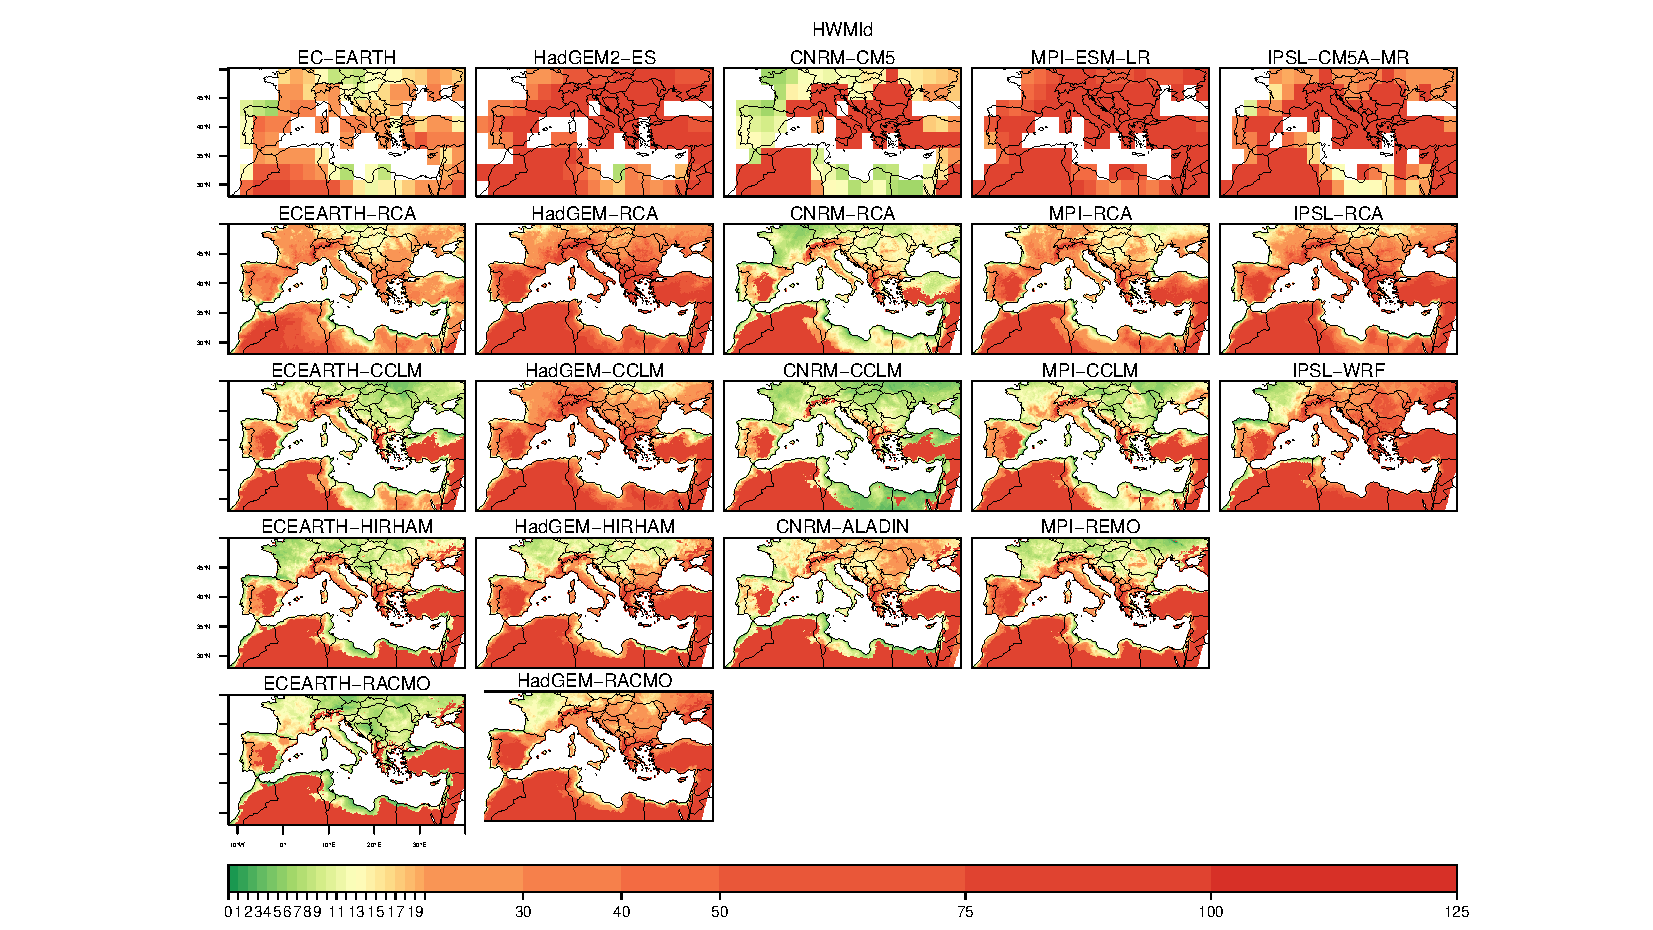
\includegraphics[width=17.0cm]{Figura3HWMIdFINAL}
\caption{Heat Wave Magnitude Index daily, averaged for the future climate period (2071-2100) for 0.11 resolution and RCP8.5
emission scenario.}
\label{fighwmid}       % Give a unique label
\end{figure}

\newpage
\begin{figure}
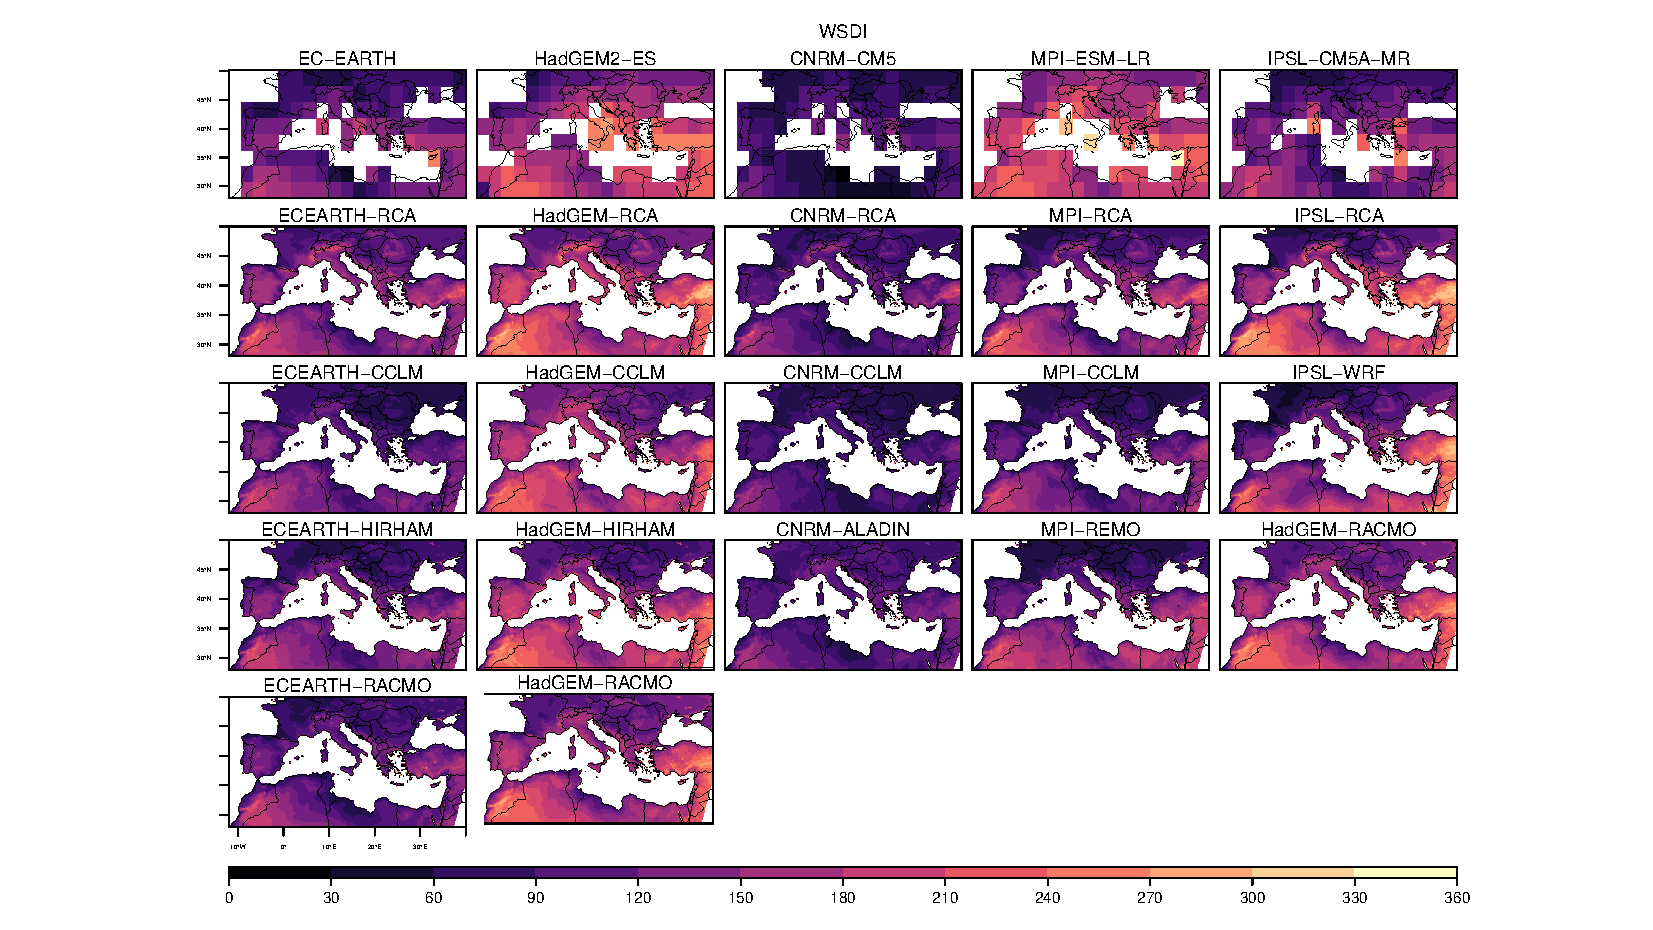
\includegraphics[width=17.0cm]{Figura3WSDIFINAL}
\caption{Warm Spell Duration Index (days/year) averaged for the future climate period (2071-2100) for 0.11 resolution and RCP8.5
emission scenario.}
\label{figwsdi}       % Give a unique label
\end{figure}

\newpage
\begin{figure}
\includegraphics[width=15.0cm]{Regiones_connombres.pdf}
\caption{Description of the nine subdomains for specific computations
made for each of the simulations. Annual regional averages will be
computed at each of these subregions: FR (France), ALPS (Alps), NEAST (North East Mediterranean), PI (Iberian Peninsula), CMED (Central Mediterranean), EAST (East Mediterranean)
WAFR (Western African coast), CAFR (Central African coast) and EAFR (Eastern African coast).}
\label{figRegiones}       % Give a unique label
\end{figure}
\newpage
\begin{figure}
\includegraphics[height=17.0cm]{printseriesHWMId}
%\begin{tabular}{ccc}
%\centering
%IP & SE & EM\\
%\includegraphics[width=.4\linewidth]{figuras/piseries}&
%\includegraphics[width=.4\linewidth]{figuras/eursseries}&
%\includegraphics[width=.4\linewidth]{figuras/medeseries}\\
%\includegraphics[width=.4\linewidth]{figuras/afrwseries}&
%\includegraphics[width=.4\linewidth]{figuras/afrseries}&\\
%WA&CA&\\
%\end{tabular}
\caption{Heat Wave Magnitude Index daily (HWMId)
averaged over each of the subregions described with its
corresponding acronym in figure \ref{figRegiones}
for each of the simulations for the whole 130 year period
ranging from 1971 to 2100 in a 5 years running window.}
\label{figseriesHWMId}
\end{figure}

\newpage
\begin{figure}
\includegraphics[height=17.0cm]{printseriesWSDI}
\caption{As \ref{figseriesHWMId} for Warm Spell Duration Index (WSDI).}
\label{figseriesWSDI}
\end{figure}


% Non-BibTeX users please use
%\begin{thebibliography}{}
%
% and use \bibitem to create references. Consult the Instructions
% for authors for reference list style.
%
%\bibitem{RefJ}
% Format for Journal Reference
%Author, Article title, Journal, Volume, page numbers (year)
% Format for books
%\bibitem{RefB}
%Author, Book title, page numbers. Publisher, place (year)
% etc
%\end{thebibliography}

\end{document}
% end of file template.tex

